\documentclass[tikz,border=10pt]{standalone}
\usepackage[utf8]{inputenc}
\usepackage{tikz}
\usepackage{mathptmx}  % Times font
\usetikzlibrary{shapes.geometric, arrows.meta, positioning, shadows, backgrounds, fit, calc}

% Define colors - Professional academic palette
\definecolor{datacolor}{RGB}{52, 152, 219}      % Blue
\definecolor{immunecolor}{RGB}{39, 174, 96}     % Green
\definecolor{analysiscolor}{RGB}{230, 126, 34}  % Orange
\definecolor{validcolor}{RGB}{155, 89, 182}     % Purple
\definecolor{resultcolor}{RGB}{22, 160, 133}    % Teal

% Define styles - REDUCED size for better page layout
\tikzstyle{modulebox} = [
    rectangle,
    rounded corners=5pt,
    minimum width=11cm,
    minimum height=1.6cm,
    text centered,
    draw=black,
    line width=1.5pt,
    drop shadow,
    fill opacity=0.15,
    text opacity=1
]

\tikzstyle{trackbox} = [
    rectangle,
    rounded corners=4pt,
    minimum width=3.3cm,
    minimum height=2.2cm,
    text centered,
    draw=black,
    line width=1.2pt,
    drop shadow={opacity=0.3},
    fill=white
]

\tikzstyle{arrow} = [
    ->,
    >=Stealth,
    line width=2pt,
    color=black!70
]

\tikzstyle{finalbox} = [
    rectangle,
    rounded corners=3pt,
    minimum width=12cm,
    minimum height=0.8cm,
    text centered,
    draw=resultcolor,
    line width=2pt,
    fill=resultcolor!20
]

\begin{document}

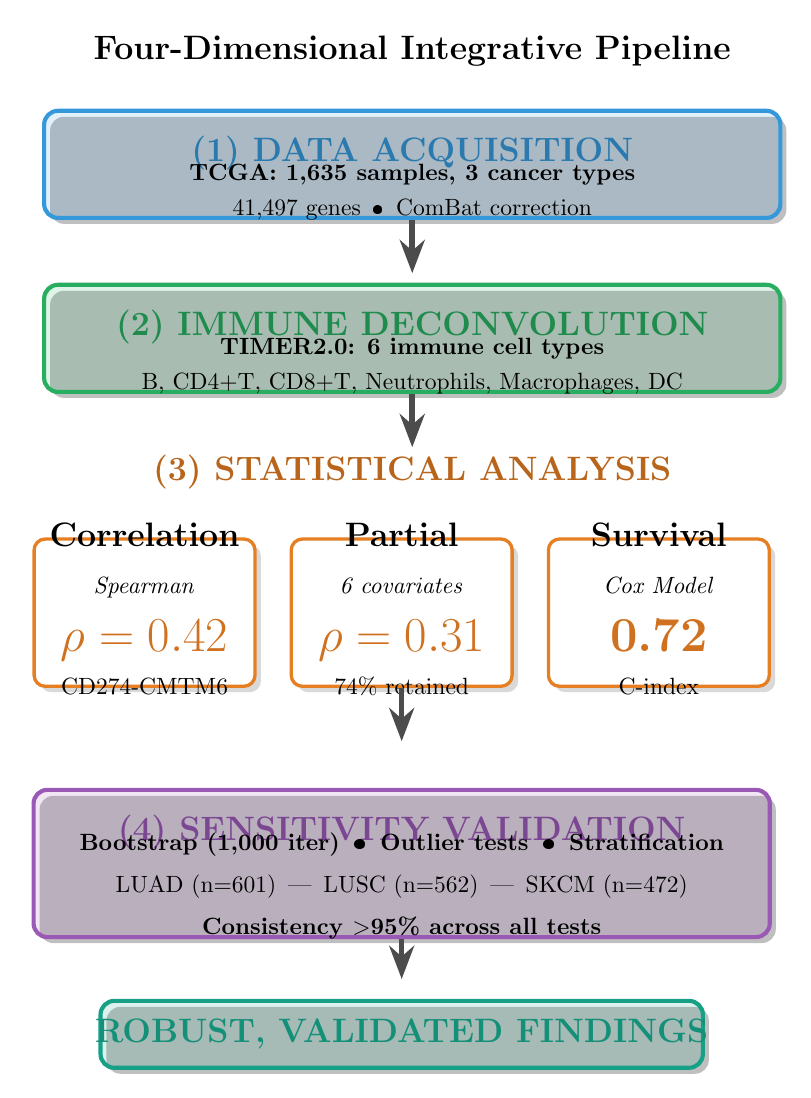
\begin{tikzpicture}[node distance=1.4cm, font=\sffamily, scale=0.85, transform shape]

% Title - Reduced size
\node[font=\Large\bfseries] (title) at (0, 9.5) {Four-Dimensional Integrative Pipeline};

% Module 1: Data Acquisition - SIMPLIFIED & REDUCED SIZE
\node[modulebox, fill=datacolor, draw=datacolor] (module1) at (0, 7.8) {};
\node[anchor=north, font=\Large\bfseries, color=datacolor!80!black] at (module1.north) [yshift=-8pt] {(1) DATA ACQUISITION};
\node[anchor=center, font=\normalsize] at (module1.center) [yshift=-12pt] {
    \begin{tabular}{c}
    \textbf{TCGA: 1,635 samples, 3 cancer types} \\[3pt]
    41,497 genes \,•\, ComBat correction
    \end{tabular}
};

% Arrow 1
\draw[arrow] (module1.south) -- ++(0, -0.8);

% Module 2: Immune Deconvolution - SIMPLIFIED & REDUCED SIZE
\node[modulebox, fill=immunecolor, draw=immunecolor] (module2) at (0, 5.2) {};
\node[anchor=north, font=\Large\bfseries, color=immunecolor!80!black] at (module2.north) [yshift=-8pt] {(2) IMMUNE DECONVOLUTION};
\node[anchor=center, font=\normalsize] at (module2.center) [yshift=-12pt] {
    \begin{tabular}{c}
    \textbf{TIMER2.0: 6 immune cell types} \\[3pt]
    B, CD4+T, CD8+T, Neutrophils, Macrophages, DC
    \end{tabular}
};

% Arrow 2
\draw[arrow] (module2.south) -- ++(0, -0.8);

% Module 3 Title - Reduced size
\node[font=\Large\bfseries, color=analysiscolor!80!black] (module3title) at (0, 3.2) {(3) STATISTICAL ANALYSIS};

% Track A - Reduced size
\node[trackbox, draw=analysiscolor, below=0.6cm of module3title, xshift=-4cm] (trackA) {};
\node[anchor=center, font=\normalsize] at (trackA.center) {
    \begin{tabular}{c}
    {\Large\bfseries Correlation} \\[8pt]
    \textit{Spearman} \\[8pt]
    {\huge\bfseries\color{analysiscolor!90!black} $\rho = 0.42$} \\[6pt]
    {\normalsize CD274-CMTM6}
    \end{tabular}
};

% Track B - Reduced size
\node[trackbox, draw=analysiscolor, right=0.5cm of trackA] (trackB) {};
\node[anchor=center, font=\normalsize] at (trackB.center) {
    \begin{tabular}{c}
    {\Large\bfseries Partial} \\[8pt]
    \textit{6 covariates} \\[8pt]
    {\huge\bfseries\color{analysiscolor!90!black} $\rho = 0.31$} \\[6pt]
    {\normalsize 74\% retained}
    \end{tabular}
};

% Track C - Reduced size
\node[trackbox, draw=analysiscolor, right=0.5cm of trackB] (trackC) {};
\node[anchor=center, font=\normalsize] at (trackC.center) {
    \begin{tabular}{c}
    {\Large\bfseries Survival} \\[8pt]
    \textit{Cox Model} \\[8pt]
    {\huge\bfseries\color{analysiscolor!90!black} 0.72} \\[6pt]
    {\normalsize C-index}
    \end{tabular}
};

% Arrow 3
\draw[arrow] (trackB.south) -- ++(0, -0.8);

% Module 4: Sensitivity Analysis - Reduced size
\node[modulebox, fill=validcolor, draw=validcolor, below=1.5cm of trackB, minimum height=2.2cm] (module4) {};
\node[anchor=north, font=\Large\bfseries, color=validcolor!80!black] at (module4.north) [yshift=-8pt] {(4) SENSITIVITY VALIDATION};
\node[anchor=center, font=\normalsize] at (module4.center) [yshift=-10pt] {
    \begin{tabular}{c}
    \textbf{Bootstrap (1,000 iter) \,•\, Outlier tests \,•\, Stratification} \\[6pt]
    LUAD (n=601) \,|\, LUSC (n=562) \,|\, SKCM (n=472) \\[6pt]
    {\normalsize\bfseries Consistency $>$95\% across all tests}
    \end{tabular}
};

% Arrow to final result
\draw[arrow] (module4.south) -- ++(0, -0.6);

% Final Result Box - with arrow connection and proper styling
\node[modulebox, fill=resultcolor, draw=resultcolor, below=0.9cm of module4, minimum height=1cm, minimum width=9cm] (result) {};
\node[anchor=center, font=\Large\bfseries, color=resultcolor!90!black] at (result.center) {
    ROBUST, VALIDATED FINDINGS
};

\end{tikzpicture}

\end{document}
